% Generated from paper/journal/manuscript_en.md and verified frozen outputs.
% Self-contained: no external figures or bibliography files required.
\documentclass[preprint,11pt,authoryear]{elsarticle}
\usepackage{geometry}
\geometry{a4paper,margin=25mm}
\usepackage[T1]{fontenc}
\usepackage{newtxtext,newtxmath,amsmath,booktabs,longtable,array}
\usepackage{tikz,pgfplots}
\pgfplotsset{compat=1.18}
\usepackage[colorlinks=true,linkcolor=blue,urlcolor=blue]{hyperref}
\usepackage{microtype}
\setlength{\parindent}{0pt}
\setlength{\parskip}{5pt}
\setlength{\emergencystretch}{3em}
\makeatletter
\let\ps@pprintTitle\ps@plain
\makeatother
\begin{document}

\begin{frontmatter}

\title{Separating repeated-item success from transfer in adaptive programming practice: An auditable learner model and reinforcement-learning study}

\begin{abstract}

Adaptive programming recommenders need to distinguish correct execution, response prediction and the value of selecting an exercise. We develop a reproducible prototype combining twelve executable Python tasks, a Bayesian learner-state filter and a Double Deep Q-Network policy. A shared catalog and numerical parity checks connect the trained policy to the application. The controlled evaluation includes seven policies, five synthetic environments, three training seeds and 31,500 rollouts involving 1,500 distinct simulated learners. Accounting for repeated-item familiarity reduces validation negative log-likelihood in all three fits. However, this predictive improvement does not consistently improve exercise selection. In nominal dynamics, the repeat-aware policy achieves 17.91 percentage points of expected transfer-probe gain, compared with 18.85 for the naive variant and 19.16 for a weakest-skill rule. The paired difference against weakest skill is -1.24 points, with a conditional 95\% interval of [-2.27, -0.21]. A repair-only negative control produces zero transfer gain despite substantial practice correctness. The study contributes an inspectable implementation and a bounded negative result: predictive gains alone do not establish recommendation value. The estimates are conditional on declared simulator assumptions and fixed trained models; they do not measure human learning effects or establish state-of-the-art performance.

\end{abstract}

\begin{keyword}

adaptive learning \sep programming education \sep knowledge tracing \sep reinforcement learning \sep simulation \sep reproducibility

\end{keyword}

\end{frontmatter}

\fontsize{11}{14.5}\selectfont

\section*{1. Introduction}

Repeated submissions are a defining feature of programming practice. A learner can repair one solution until it passes a test suite, yet remain unable to solve an unfamiliar task that requires the same underlying idea. An exercise recommender therefore faces a measurement problem: successful execution, predictable responses and transferable learning are related quantities with different meanings. Optimizing one does not automatically optimize the others.

Knowledge tracing supplies a history-dependent representation for personalization, but its usual predictive target is a subsequent observed response. The educational decision is different: which eligible exercise should the learner attempt next? The distinction is consequential when repetition improves item-specific familiarity, when knowledge states are imperfectly estimated, or when the reward favors immediate correctness. A complete implementation must also preserve the identity of the exercise on which a model was trained when that model is used in an application.

We address these issues with an executable research prototype and a controlled simulator benchmark. The application grades authored Python tasks, updates a learner-state estimate and selects a subsequent task through a learned policy. The benchmark separates practice responses from independent, unpractised probes. Historical programming-log forecasting is retained as separate evidence; those logs do not provide matched trajectories for the authored task bank and are not used to claim that the deployed recommender improves human learning.

The investigation asks three questions. RQ1: Does explicitly representing repeated-item familiarity improve next-response prediction? RQ2: Does this improvement produce higher transfer-oriented policy value under a fixed training budget? RQ3: How sensitive are the conclusions to the reward and to changes in the simulated learning process?

The contributions are: an auditable connection between executable tasks and learned selection; a controlled comparison that retains unsuccessful as well as favorable contrasts; and a reproducible reporting path from frozen rollout records to application traces, tables and figures. Neither the Bayesian filter nor Double DQN is proposed as a new algorithm. The contribution is an implementation and evaluation study with a clearly delimited claim, rather than a claim of superior tutoring effectiveness.

\section*{2. Related work}

Knowledge tracing originated as a model of procedural knowledge acquisition (Corbett \& Anderson, 1994). Deep Knowledge Tracing instead represents response histories through recurrent neural networks (Piech et al., 2015). Minn (2022) discusses how knowledge assessment depends on the student model, domain representation and available observations. These distinctions motivate our separation of observed correctness, model beliefs and policy outcomes. They do not establish that our three author-assigned skill groups measure human cognitive constructs.

Programming-specific models can exploit information inside the submitted program. Code-DKT augments correctness histories with code-derived features (Shi et al., 2022). Our application executes code to provide feedback, but the learner-state model consumes only the item identifier and binary whole-task outcome. The program, number of passed cases, hint use and time spent writing are not model features. This choice makes the current information boundary explicit and leaves code-aware diagnosis as an extension.

Exercise recommendation already combines knowledge tracing and reinforcement learning. ExRec integrates question semantics, knowledge tracing and policy optimization (Ozyurt et al., 2025). UniER provides a common benchmark for item-level and path-level recommendation (Cheng et al., 2026). These works rule out novelty claims based simply on combining a student model with an RL algorithm. Our comparison is restricted to the seven implemented policies under a common local protocol; ExRec and UniER were reviewed but not reproduced, and their reported scores are not directly comparable to ours.

Girard et al. (2026) investigate adaptive instructional policies using logged interactions and a contextual-bandit formulation. Such work is relevant when prospective intervention is unavailable, but an offline policy-value estimate requires justified modeling and evaluation assumptions. Matched histories and assignment propensities for our twelve tasks are unavailable. We consequently use explicit simulation for policy evaluation and retain observational forecasting claims separately. Double DQN is used as an established value-based learning method (van Hasselt et al., 2016).

\section*{3. System and problem formulation}

\subsection*{3.1. Task bank and information boundary}

The bank contains 12 Python tasks and 96 executable reference cases. Each task has a statement, examples, starter function, hints, test cases, an author-assigned primary skill and a difficulty level. The skill groups are selection and accumulation, memory and data structures, and state updates. The shared catalog supplies the same task identifiers and action order to training and browser inference. A SHA-256 mismatch disables learned selection. This establishes software compatibility, not transfer from a simulator to a human population.

Figure 1 summarizes training and application operation. At decision time, the recommender uses only observations already available in the chronological history. Passed and failed grading outcomes are included; identical source code for the same task contributes at most one model observation. Execution errors, cancellation and malformed observations are excluded. The displayed number of passed tests remains feedback from the grader, whereas the model target is binary success on the entire task.

\begin{figure}[htbp]\centering

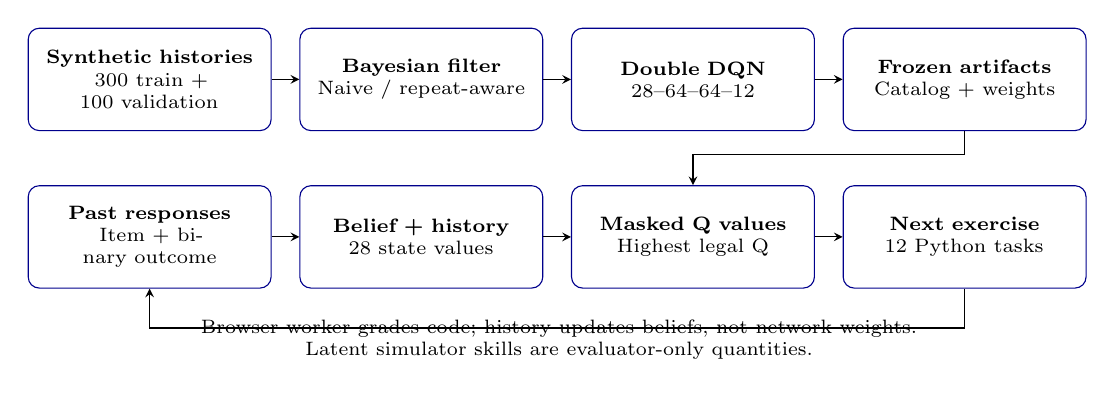
\begin{tikzpicture}[>=stealth, every node/.style={font=\scriptsize}, box/.style={draw=blue!55!black,rounded corners,align=center,text width=2.85cm,minimum height=1.3cm}]
\node[box] (n00) at (0.00,0.00) {\textbf{Synthetic histories}\\300 train + 100 validation};
\node[box] (n01) at (3.45,0.00) {\textbf{Bayesian filter}\\Naive / repeat-aware};
\draw[->] (n00) -- (n01);
\node[box] (n02) at (6.90,0.00) {\textbf{Double DQN}\\28--64--64--12};
\draw[->] (n01) -- (n02);
\node[box] (n03) at (10.35,0.00) {\textbf{Frozen artifacts}\\Catalog + weights};
\draw[->] (n02) -- (n03);
\node[box] (n10) at (0.00,-2.00) {\textbf{Past responses}\\Item + binary outcome};
\node[box] (n11) at (3.45,-2.00) {\textbf{Belief + history}\\28 state values};
\draw[->] (n10) -- (n11);
\node[box] (n12) at (6.90,-2.00) {\textbf{Masked Q values}\\Highest legal Q};
\draw[->] (n11) -- (n12);
\node[box] (n13) at (10.35,-2.00) {\textbf{Next exercise}\\12 Python tasks};
\draw[->] (n12) -- (n13);
\draw[->] (n03.south) -- ++(0,-.3) -| (n12.north);
\draw[->] (n13.south) -- ++(0,-.5) -| (n10.south);
\node[align=center] at (5.2,-3.3) {Browser worker grades code; history updates beliefs, not network weights.\\Latent simulator skills are evaluator-only quantities.};
\end{tikzpicture}

\caption{Training artifacts and browser decision flow. Only retained past responses enter the learner-state update. The application does not observe latent simulator skills.}\end{figure}

The system does not infer psychological mastery from a test count. Its three belief values are internal model variables with a synthetic prior of 0.3. A new user receives a prior-based recommendation, which is explicitly labeled as lacking individual evidence. New observations update the state; browser interactions do not retrain the policy weights.

\subsection*{3.2. Belief-state representation}

Let b(k) denote the current belief for skill k, n(a) the previous count for task a, z(a) its solved flag and t the number of retained observations. The policy input contains 28 values: three beliefs, twelve capped counts divided by three, twelve solved flags and the remaining episode budget divided by twelve. A finite belief representation approximates a partially observed decision process; it is not proof that human learning is Markovian.

For every observation, the filter first applies forgetting f = 0.005 to all beliefs. The active skill then receives a learning transition with rate l(1 + 0.15d), where d is the authored difficulty. Item familiarity is rho = m(1 - exp(-n(a))). The response emissions for a learned and unlearned skill are shown in Equation 1; g, s and m are fitted guess, slip and familiarity parameters.

\begin{equation}\begin{gathered}q_1=1-s-0.05d+(s+0.05d)\rho,\q_0=g-0.05d+(1-g+0.05d)\rho.\end{gathered}\tag{1}\end{equation}

If b* is the active belief after its transition, the predicted response probability is p = b*q1 + (1 - b*)q0. After observing y, the active belief receives the Bayesian update in Equation 2; other beliefs retain their forgetting update. Prediction precedes use of the current response label.

\begin{equation}\begin{gathered}b^{+}=\frac{b^{*}q_1^{y}(1-q_1)^{1-y}}{p^{y}(1-p)^{1-y}}.\end{gathered}\tag{2}\end{equation}

The naive filter fixes familiarity at zero. The repeat-aware filter searches m in \{0, 0.4, 0.7\}; both search learning in \{0.04, 0.10, 0.16\}, guess in \{0.16, 0.24\} and slip in \{0.08, 0.16\}. Each fit minimizes training response negative log-likelihood over this fixed grid. Validation is descriptive and is not used to select a checkpoint after examining policy outcomes.

\subsection*{3.3. Action space, reward and Double DQN}

An action selects a specific task. The legal action set excludes solved tasks and tasks with three prior retained observations. The greedy policy selects the highest Q value among legal actions, breaking ties by action order. The 28-64-64-12 network has 6,796 parameters and rectified linear hidden layers. Double DQN separates action selection by the online network from value evaluation by the target network, as in Equation 3.

\begin{equation}\begin{gathered}a^{*}=\operatorname{argmax}_{a\in\mathcal{A}(x^{\prime})}Q_{\theta}(x^{\prime},a),\Y=r+\gamma(1-\mathrm{done})Q_{\bar{\theta}}(x^{\prime},a^{*}).\end{gathered}\tag{3}\end{equation}

Table 1 reports the training and evaluation settings. All networks use a fixed 24,000-transition budget, rather than a checkpoint chosen for favorable test performance. Nine networks are trained: naive/probe, aware/probe and aware/correctness, each with seeds 101, 203 and 307. The probe reward combines a per-step cost of -0.005c(a) and the sampled fraction correct on twelve independent terminal probes. Four probes correspond to each skill and contain no familiarity bonus. The correctness ablation replaces the terminal probe reward with y/12 at each practice step.

\begingroup\small\setlength{\tabcolsep}{3pt}

\begin{longtable}{p{0.373\textwidth}p{0.579\textwidth}}

\multicolumn{2}{l}{\textbf{Table 1.} Training and evaluation settings}\\

\toprule

\textbf{Setting / Cấu hình} & \textbf{Value / Giá trị}\\\midrule\endfirsthead

\textbf{Setting / Cấu hình} & \textbf{Value / Giá trị}\\\midrule\endhead

\bottomrule\endfoot

Catalog / executable tests & 12 tasks / 96 cases\\

History length / attempt cap & 12 / 3\\

Filter histories per seed & 300 train; 100 validation\\

Training seeds & 101, 203, 307\\

Network / parameters & 28-64-64-12 ReLU / 6,796\\

Transitions / networks & 24,000 per network / 9 networks\\

Replay / batch / warm-up & 12,000 / 64 / 512 transitions\\

Update / target copy & Every 4 / 400 transitions\\

Optimizer / learning rate & Adam / 0.001; Huber loss; norm clip 5\\

Discount / exploration & 0.99; epsilon 1 to 0.05 over 75\% of budget\\

Evaluation & 7 policies; 5 worlds; 300 learners/world\\

Sampling / intervals & 1,500 learner identities; 1,500 paired bootstraps\\

Recorded framework & PyTorch 2.12.0+cpu; one CPU thread\\

\end{longtable}\endgroup

The cost c(a) = 1 + 0.2d is an authored simulation assumption, not measured student solution time. The policy observes sampled response outcomes and reward, not the simulator's hidden mastery. The learner model is fitted separately and held fixed during policy training. Policy and filter errors can therefore affect the resulting behavior, even when the representation has a lower response-prediction loss.

\section*{4. Experimental design}

\subsection*{4.1. Environments and data partitions}

The simulator represents three binary latent skills. Nominal dynamics use learning 0.10, familiarity 0.60 and forgetting 0.005, with difficulty-dependent learning and response emissions. We evaluate five declared environments: nominal, repair-only, slow transfer, increased forgetting and prerequisites. Repair-only sets learning and forgetting to zero while increasing familiarity to 0.80. Slow transfer reduces learning to 0.025; increased forgetting raises forgetting to 0.05. The prerequisite environment reduces the learning rate by a factor of ten when the preceding skill is absent. These are authored stress tests, not empirically calibrated models of student behavior.

For each training seed, the filter uses 300 synthetic training histories and 100 separate validation histories, each containing twelve interactions. Policy training uses a separate seed namespace and nominal dynamics. Evaluation uses 300 new learner seeds in each environment, shared across policies and training fits to enable paired comparisons. Figure 2 makes the sampling unit and the measurement boundary explicit.

\begin{figure}[htbp]\centering

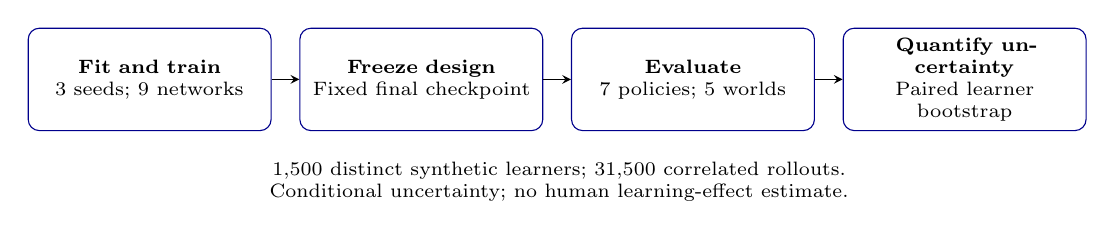
\begin{tikzpicture}[>=stealth, every node/.style={font=\scriptsize}, box/.style={draw=blue!55!black,rounded corners,align=center,text width=2.85cm,minimum height=1.3cm}]
\node[box] (n00) at (0.00,0.00) {\textbf{Fit and train}\\3 seeds; 9 networks};
\node[box] (n01) at (3.45,0.00) {\textbf{Freeze design}\\Fixed final checkpoint};
\draw[->] (n00) -- (n01);
\node[box] (n02) at (6.90,0.00) {\textbf{Evaluate}\\7 policies; 5 worlds};
\draw[->] (n01) -- (n02);
\node[box] (n03) at (10.35,0.00) {\textbf{Quantify uncertainty}\\Paired learner bootstrap};
\draw[->] (n02) -- (n03);
\node[align=center] at (5.2,-1.3) {1,500 distinct synthetic learners; 31,500 correlated rollouts.\\Conditional uncertainty; no human learning-effect estimate.};
\end{tikzpicture}

\caption{Fixed-design experiment and sampling units. Repeated rollouts share learner seeds and trained fits; they are not independent human participants.}\end{figure}

The total of 31,500 rollouts is 7 policies \ensuremath{\times} 5 environments \ensuremath{\times} 3 fits \ensuremath{\times} 300 learners. It comprises 1,500 distinct simulated learner identities, not 31,500 independent students. Source, input hashes, design, commands and outputs are stored in the frozen run. Earlier v1 results had already been inspected and informed v2. The v2 design was recorded before its own evaluation, but this local record is not external preregistration. The reported v2 results are now inspected.

\subsection*{4.2. Comparators and outcomes}

The four non-RL comparators select an eligible task randomly, by increasing authored difficulty, by the weakest estimated skill, or by predicted response probability closest to 0.7. The last is a heuristic comparator, not a validated operationalization of the zone of proximal development. The three learned variants provide encoder and reward comparisons under the same fixed interaction budget.

The primary outcome is the change in expected success on an independent transfer probe, defined in Equation 4. Only the held-out evaluator reads latent mastery M to compute this low-noise expectation. The term “transfer” therefore denotes an explicitly defined simulator quantity; it does not denote an observed human transfer test. Practice correctness, final expected probe score, sampled terminal probe score and cost are retained separately.

\begin{equation}\begin{gathered}G=\frac{1}{3}\sum_{k=1}^{3}[(0.2+0.7M_{T,k})-(0.2+0.7M_{0,k})].\end{gathered}\tag{4}\end{equation}

For each simulated learner, we average the outcome over the three fixed fitted models. We then resample learners, preserving policy pairing, for 1,500 percentile bootstrap replicates. The 95\% intervals are conditional on those fitted models and do not cover all possible retraining variability. The primary contrast is aware/probe minus naive/probe in each environment; weakest-skill and reward-ablation contrasts are secondary. Multiple comparisons are reported without a multiplicity adjustment and interpreted as exploratory.

\section*{5. Results}

\subsection*{5.1. Prediction improves, selection does not necessarily improve}

Table 2 gives every filter-validation result. Repeat-aware modeling reduces validation negative log-likelihood in all three fits. Figure 3 presents this predictive change alongside policy value, using separate axes and units to avoid equating the two measurements.

\begingroup\small\setlength{\tabcolsep}{3pt}

\begin{longtable}{p{0.110\textwidth}p{0.247\textwidth}p{0.271\textwidth}p{0.275\textwidth}}

\multicolumn{4}{l}{\textbf{Table 2.} Validation negative log-likelihood per response}\\

\toprule

\textbf{Seed} & \textbf{Naive} & \textbf{Repeat-aware} & \textbf{Aware - naive}\\\midrule\endfirsthead

\textbf{Seed} & \textbf{Naive} & \textbf{Repeat-aware} & \textbf{Aware - naive}\\\midrule\endhead

\bottomrule\endfoot

101 & 0.637583 & 0.622301 & -0.015281\\

203 & 0.643206 & 0.631533 & -0.011672\\

307 & 0.653636 & 0.621808 & -0.031827\\

\end{longtable}\endgroup

In nominal dynamics, the aware/probe policy achieves 17.91 percentage points of expected transfer-probe gain, compared with 18.85 for naive/probe and 19.16 for weakest skill (Table 3). Its difference from naive/probe is -0.93 points with interval [-1.87, -0.05], and its difference from weakest skill is -1.24 points with interval [-2.27, -0.21]. These contrasts do not support superiority of the repeat-aware policy under the tested budget. They also do not establish that a different training budget or representation would produce the same ranking.

\begingroup\small\setlength{\tabcolsep}{3pt}

\begin{longtable}{p{0.366\textwidth}p{0.108\textwidth}p{0.258\textwidth}p{0.171\textwidth}}

\multicolumn{4}{l}{\textbf{Table 3.} Nominal policy outcomes}\\

\toprule

\textbf{Policy} & \textbf{Gain (pp)} & \textbf{95\% CI (pp)} & \textbf{Practice (\%)}\\\midrule\endfirsthead

\textbf{Policy} & \textbf{Gain (pp)} & \textbf{95\% CI (pp)} & \textbf{Practice (\%)}\\\midrule\endhead

\bottomrule\endfoot

Random & 16.96 & [14.86, 19.13] & 51.69\\

Difficulty order & 16.64 & [14.50, 18.90] & 54.75\\

Weakest skill & 19.16 & [17.07, 21.40] & 50.76\\

Target p = 0.7 & 14.16 & [12.13, 16.24] & 59.72\\

DDQN naive / probe & 18.85 & [16.83, 20.97] & 54.29\\

DDQN aware / probe & 17.91 & [15.90, 20.03] & 53.61\\

DDQN aware / correct & 17.24 & [15.30, 19.37] & 56.16\\

\end{longtable}\endgroup

The probability-target heuristic has the highest mean practice correctness in this environment, 59.72\%, but lower transfer-probe gain than the other reported policies. This illustrates why a practice-success metric cannot replace the declared policy objective in this simulator. It is not evidence that targeting a particular human success rate is generally harmful.

\begin{figure}[htbp]\centering

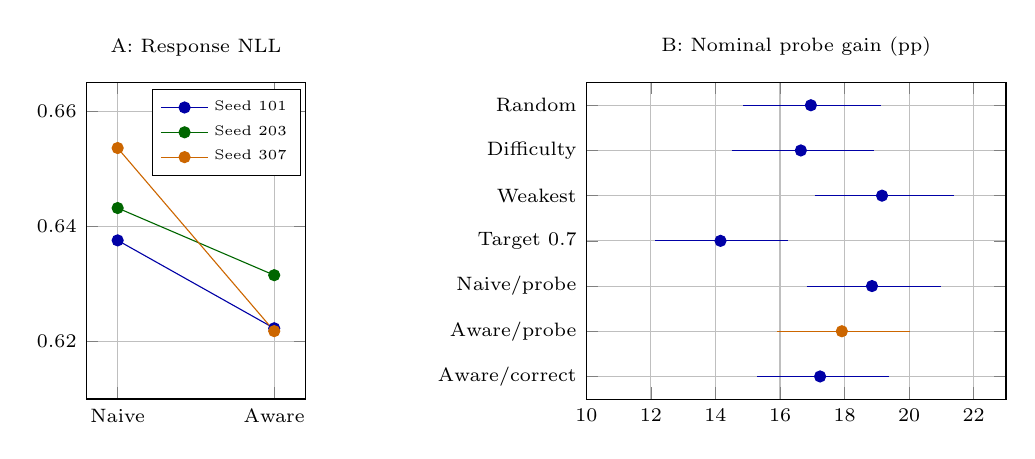
\begin{tikzpicture}
\begin{axis}[width=.36\textwidth,height=5.6cm,title={A: Response NLL},xtick={0,1},xticklabels={Naive,Aware},xmin=-.2,xmax=1.2,ymin=.61,ymax=.665,grid=major,font=\scriptsize,legend style={font=\tiny,at={(.98,.98)},anchor=north east}]
\addplot[color=blue!65!black,mark=*] coordinates {(0,0.63758258) (1,0.62230123)};\addlegendentry{Seed 101}
\addplot[color=green!40!black,mark=*] coordinates {(0,0.64320558) (1,0.63153337)};\addlegendentry{Seed 203}
\addplot[color=orange!80!black,mark=*] coordinates {(0,0.65363582) (1,0.62180848)};\addlegendentry{Seed 307}
\end{axis}
\begin{axis}[at={(6.35cm,0)},anchor=south west,width=.57\textwidth,height=5.6cm,title={B: Nominal probe gain (pp)},xmin=10,xmax=23,ymin=-.5,ymax=6.5,y dir=reverse,ytick={0,1,2,3,4,5,6},yticklabels={Random,Difficulty,Weakest,Target 0.7,Naive/probe,Aware/probe,Aware/correct},grid=major,font=\scriptsize]
\addplot[color=blue!65!black,mark=none] coordinates {(14.855556,0) (19.133333,0)};
\addplot[color=blue!65!black,only marks,mark=*] coordinates {(16.955556,0)};
\addplot[color=blue!65!black,mark=none] coordinates {(14.503611,1) (18.900000,1)};
\addplot[color=blue!65!black,only marks,mark=*] coordinates {(16.644444,1)};
\addplot[color=blue!65!black,mark=none] coordinates {(17.071574,2) (21.403796,2)};
\addplot[color=blue!65!black,only marks,mark=*] coordinates {(19.159259,2)};
\addplot[color=blue!65!black,mark=none] coordinates {(12.132037,3) (16.243241,3)};
\addplot[color=blue!65!black,only marks,mark=*] coordinates {(14.155556,3)};
\addplot[color=blue!65!black,mark=none] coordinates {(16.825926,4) (20.974074,4)};
\addplot[color=blue!65!black,only marks,mark=*] coordinates {(18.848148,4)};
\addplot[color=orange!80!black,mark=none] coordinates {(15.904907,5) (20.028426,5)};
\addplot[color=orange!80!black,only marks,mark=*] coordinates {(17.914815,5)};
\addplot[color=blue!65!black,mark=none] coordinates {(15.296296,6) (19.366667,6)};
\addplot[color=blue!65!black,only marks,mark=*] coordinates {(17.240741,6)};
\end{axis}
\end{tikzpicture}

\caption{Prediction and selection have different outcomes. A: validation negative log-likelihood, lower is better. B: nominal expected probe gain; bars show 95\% learner-bootstrap intervals conditional on three fixed fits.}\end{figure}

\subsection*{5.2. Stress tests and reward comparison}

Figure 4 reports every environment for the three paired contrasts. The direction of the encoder comparison changes under prerequisites: aware/probe minus naive/probe is 1.19 points with interval [0.16, 2.20]. The comparison with weakest skill in that environment includes zero. Under increased forgetting, aware/probe exceeds its correctness-reward ablation by 2.10 points with interval [1.18, 3.00]. These results are compatible with environment-sensitive policy rankings; they do not isolate a single causal explanation inside the trained networks.

\begin{figure}[htbp]\centering

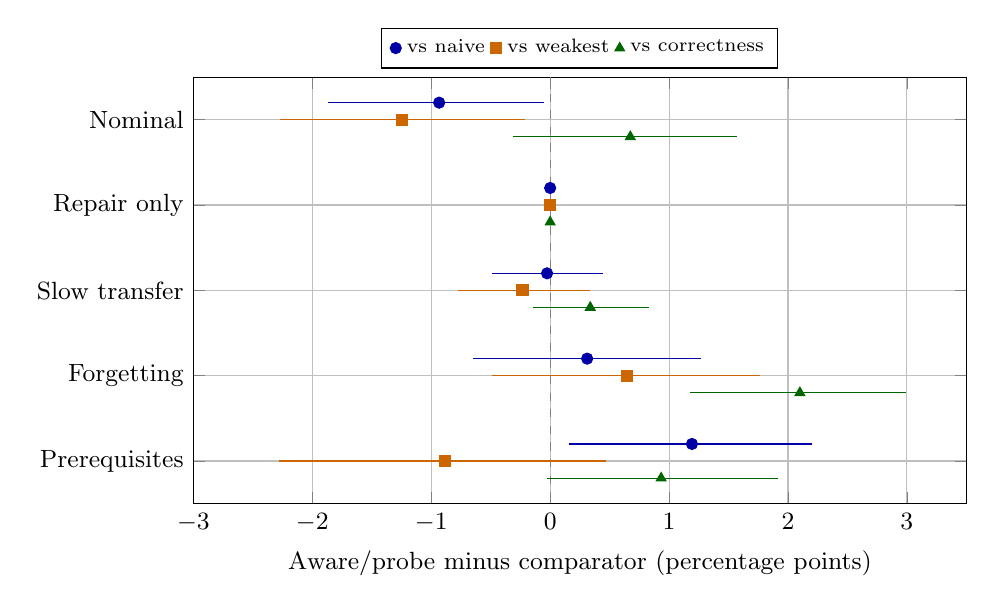
\begin{tikzpicture}
\begin{axis}[width=.94\textwidth,height=7cm,xmin=-3,xmax=3.5,ymin=-.5,ymax=4.5,y dir=reverse,ytick={0,1,2,3,4},yticklabels={Nominal,Repair only,Slow transfer,Forgetting,Prerequisites},xlabel={Aware/probe minus comparator (percentage points)},grid=major,font=\small,legend style={font=\scriptsize,at={(.5,1.02)},anchor=south,legend columns=3}]
\addplot[gray,dashed,forget plot] coordinates {(0,-.5) (0,4.5)};
\addplot[color=blue!65!black,mark=none,forget plot] coordinates {(-1.866667,-0.20) (-0.051852,-0.20)};
\addplot[color=blue!65!black,mark=none,forget plot] coordinates {(0.000000,0.80) (0.000000,0.80)};
\addplot[color=blue!65!black,mark=none,forget plot] coordinates {(-0.492593,1.80) (0.440741,1.80)};
\addplot[color=blue!65!black,mark=none,forget plot] coordinates {(-0.648148,2.80) (1.270370,2.80)};
\addplot[color=blue!65!black,mark=none,forget plot] coordinates {(0.155556,3.80) (2.203704,3.80)};
\addplot[color=blue!65!black,only marks,mark=*] coordinates {(-0.933333,-0.20) (0.000000,0.80) (-0.025926,1.80) (0.311111,2.80) (1.192593,3.80)};\addlegendentry{vs naive}
\addplot[color=orange!80!black,mark=none,forget plot] coordinates {(-2.269167,0.00) (-0.207407,0.00)};
\addplot[color=orange!80!black,mark=none,forget plot] coordinates {(0.000000,1.00) (0.000000,1.00)};
\addplot[color=orange!80!black,mark=none,forget plot] coordinates {(-0.777778,2.00) (0.337037,2.00)};
\addplot[color=orange!80!black,mark=none,forget plot] coordinates {(-0.492593,3.00) (1.762963,3.00)};
\addplot[color=orange!80!black,mark=none,forget plot] coordinates {(-2.281481,4.00) (0.466667,4.00)};
\addplot[color=orange!80!black,only marks,mark=square*] coordinates {(-1.244444,0.00) (0.000000,1.00) (-0.233333,2.00) (0.648148,3.00) (-0.881481,4.00)};\addlegendentry{vs weakest}
\addplot[color=green!40!black,mark=none,forget plot] coordinates {(-0.311111,0.20) (1.569167,0.20)};
\addplot[color=green!40!black,mark=none,forget plot] coordinates {(0.000000,1.20) (0.000000,1.20)};
\addplot[color=green!40!black,mark=none,forget plot] coordinates {(-0.143241,2.20) (0.829630,2.20)};
\addplot[color=green!40!black,mark=none,forget plot] coordinates {(1.178981,3.20) (2.995093,3.20)};
\addplot[color=green!40!black,mark=none,forget plot] coordinates {(-0.025926,4.20) (1.918519,4.20)};
\addplot[color=green!40!black,only marks,mark=triangle*] coordinates {(0.674074,0.20) (0.000000,1.20) (0.337037,2.20) (2.100000,3.20) (0.933333,4.20)};\addlegendentry{vs correctness}
\end{axis}
\end{tikzpicture}

\caption{Paired probe-gain contrasts across all five environments. Points compare aware/probe with each named comparator. Bars are conditional 95\% intervals; zero means no observed mean difference. No multiplicity adjustment is applied.}\end{figure}

In repair-only dynamics, gain is zero for every policy by construction, although practice correctness ranges from 43.75\% to 54.86\%. The result checks that the implementation can distinguish familiarity-driven success from the chosen transfer measure. The environment deliberately has no new learning; the result must not be described as a discovery that real students cannot learn by retrying. Appendix A retains all 35 policy-environment rows, including zero and unfavorable outcomes, while the companion CSV files provide unrounded means, intervals, fitted parameters and paired contrasts.

\section*{6. Application verification}

The deployed member is the aware/probe network with seed 101, selected in the protocol before policy evaluation for demonstration. It is not the best-performing policy identified after inspection. Python executes inside a disposable local browser worker; the application supplies concrete test feedback, preserves drafts and exports the decision history. A separate research view compares hypothetical histories without editing personal practice records.

Numerical parity fixtures compare Python and JavaScript belief updates, response predictions and Q values. The maximum observed Q difference is 8.05e-08, below the 0.000002 tolerance; belief and probability differences are zero for the five fixtures. The operational regression includes 40 harness, policy and backend checks, and all 96 reference cases in browser Python. Additional rehearsals cover Chromium, Edge and Chrome, local-only networking, missing-resource recovery and restart of a test-owned server. These checks establish the tested software behavior rather than pedagogical effectiveness or exhaustive correctness for every possible program.

The learned policy has a finite operating scope. Twelve retained observations, excessive attempts on one task, a new observation after a task was solved, no eligible action, or unavailable/incompatible artifacts trigger an explicitly labeled rule fallback. Repeating a solved task manually remains possible. The policy-value tables do not evaluate an unlimited mixture of learned and fallback recommendations in human use.

\section*{7. Discussion and limitations}

\subsection*{7.1. Interpretation of the negative result}

The central finding concerns measurement alignment. Familiarity is useful for predicting repeated-item responses, but a policy trained through that representation must also learn to select actions that advance the chosen objective. Improved likelihood does not by itself certify that this downstream optimization succeeds. A transparent heuristic remains a demanding comparator in the nominal experiment, and retaining that result prevents a prediction gain from being promoted into an unsupported recommendation claim.

The study does not show that repeat-aware models are intrinsically worse, that reinforcement learning is unnecessary, or that the weakest-skill rule is universally optimal. Only three fitted models and one fixed interaction budget were evaluated. No convergence study, broad hyperparameter search or sensitivity analysis over skill mappings was completed. The intervals are conditional and the several comparisons are exploratory.

\subsection*{7.2. Construct and external validity}

Latent skills, item difficulties, costs and learning mechanisms are authored assumptions. The fitted model shares part of the simulator's structure, and the five environments cannot represent every source of misspecification. Catalog identity checks validate task mapping in software, not a psychological interpretation of the skill variables. Twelve introductory tasks are not a representative programming curriculum, and passing their finite tests does not demonstrate general problem-solving ability.

The filter does not model source-code semantics, partial test success, hint use, elapsed writing time or forgetting over calendar days. A learner who copies a solution can produce a passing response without the learning implied by a naive interpretation of correctness. Those omitted factors limit use of the current belief values as student-facing diagnostic scores. In particular, the simulated cost does not satisfy an empirical claim of improved human solution time.

No prospective student intervention or validated human off-policy value estimate was obtained. The historical ACcoding forecasting component concerns a fixed logged next task, not the effect of selecting a different one. It cannot validate this authored-bank policy. Modern external recommendation baselines have not been reproduced under a common benchmark, so no claim of algorithmic novelty, SOTA performance or publication-tier readiness follows from the present results.

\subsection*{7.3. Research and design implications}

Future evaluation should use public data with genuinely matched tasks and histories, validate skill annotations, and test modern recommendation baselines under a common protocol. A simulator should be fitted and checked against external observations before stronger claims about real learning are made. Any follow-up selected after seeing these results needs a newly declared protocol. These directions do not require an unplanned claim that a student trial has already occurred.

For system design, the practical implication is to expose the provenance and scope of each displayed quantity. Test correctness is executable feedback; predicted success is a model output; belief is an internal state; and transfer-probe gain is a simulator evaluation target. Keeping these meanings distinct makes a demonstration inspectable without converting its visual plausibility into evidence of learning impact.

\section*{8. Conclusion}

The prototype connects executable programming tasks to learner-state updates and learned exercise selection. Its controlled experiment finds better repeat-aware response likelihood in every fitted seed, but no corresponding nominal advantage over the naive policy or weakest-skill comparator. Independent probes, stress tests, artifact checks and software rehearsals make the claim auditable. The demonstrated result is a functioning implementation and a bounded simulator finding; human learning effectiveness remains unestablished.

\section*{Data and code availability}

The local artifact contains the catalog, nine trained networks, protocol and source snapshots, rollout arrays, aggregate summaries, decision traces and reporting scripts. It has not been assigned a public archive DOI, and this draft does not imply that the artifact is already publicly deposited. Raw historical learner records are excluded from the new application bundle. The reporting pipeline verifies the frozen run, checks aggregate means against rollout arrays and regenerates figures and editable tables without refitting a model. The recorded experiment took 482.0 seconds on the available CPU environment; this is not a hardware-comparable efficiency benchmark.

\section*{Ethics and disclosure status}

The policy experiment uses synthetic learners, and software verification uses disposable test histories. No new student intervention was conducted. Historical public-log work is a separate component and does not provide evidence of informed consent, institutional approval or an exemption for this manuscript. Any applicable institutional determination, funding statement, competing-interest declaration and author-contribution statement require confirmation by the human authors before submission; none is invented here.

\section*{Declaration of generative AI and AI-assisted technologies}

OpenAI Codex assisted with programming, experiment automation, literature retrieval, manuscript drafting and reproducible plotting code. Numerical results are read from recorded artifacts. Figures are deterministic vector plots and diagrams produced by code; they are not image-model renderings. Final human review of all claims, references, declarations and the journal's current AI policy remains required before submission. This working draft does not represent that such review has already been completed.

\section*{References}

\begin{list}{}{\setlength{\leftmargin}{1.3em}\setlength{\itemindent}{-1.3em}}

\item Cheng, X., Zhuang, G., Xie, Y., Wang, J., Liu, Y., Guan, Q., Fang, L., \& Pan, S. (2026). \textit{UniER: A unified benchmark for item-level and path-level exercise recommendation} [Preprint]. arXiv. \url{https://arxiv.org/abs/2605.16750}.

\item Corbett, A. T., \& Anderson, J. R. (1994). Knowledge tracing: Modeling the acquisition of procedural knowledge. \textit{User Modeling and User-Adapted Interaction, 4}, 253-278. \url{https://doi.org/10.1007/BF01099821}.

\item Girard, S., Minn, S., Bouzeghoub, A., \& Vie, J.-J. (2026). \textit{Counterfactual learning of new adaptive instructional policies using logged data} [Preprint]. arXiv. \url{https://arxiv.org/abs/2606.23015}.

\item Minn, S. (2022). AI-assisted knowledge assessment techniques for adaptive learning environments. \textit{Computers and Education: Artificial Intelligence, 3}, Article 100050. \url{https://doi.org/10.1016/j.caeai.2022.100050}.

\item Ozyurt, Y., Almaci, T., Feuerriegel, S., \& Sachan, M. (2025). Personalized exercise recommendation with semantically-grounded knowledge tracing. \textit{Advances in Neural Information Processing Systems, 38}. \url{https://proceedings.neurips.cc/paper_files/paper/2025/hash/13707aad517ddd6c09ea02e0f55e1e7a-Abstract-Conference.html}.

\item Piech, C., Spencer, J., Huang, J., Ganguli, S., Sahami, M., Guibas, L., \& Sohl-Dickstein, J. (2015). Deep knowledge tracing. \textit{Advances in Neural Information Processing Systems, 28}. \url{https://arxiv.org/abs/1506.05908}.

\item Shi, Y., Chi, M., Barnes, T., \& Price, T. W. (2022). \textit{Code-DKT: A code-based knowledge tracing model for programming tasks} [Preprint]. arXiv. \url{https://arxiv.org/abs/2206.03545}.

\item van Hasselt, H., Guez, A., \& Silver, D. (2016). Deep reinforcement learning with double Q-learning. \textit{Proceedings of the AAAI Conference on Artificial Intelligence, 30}(1), 2094-2100. \url{https://doi.org/10.1609/aaai.v30i1.10295}.

\end{list}

\clearpage

\section*{Appendix A. Complete policy outcomes}

The table preserves the full design instead of selecting only favorable environments. Gain and confidence intervals are in percentage points; practice correctness is a percentage. Intervals are conditional paired-learner bootstrap intervals, with three fixed fitted models and 300 learners per environment. The companion tables include the unrounded quantities and all paired contrasts.

\begingroup\small\setlength{\tabcolsep}{3pt}

\begin{longtable}{p{0.130\textwidth}p{0.278\textwidth}p{0.084\textwidth}p{0.221\textwidth}p{0.167\textwidth}}

\multicolumn{5}{l}{\textbf{Table A.1.} Complete policy-environment outcomes}\\

\toprule

\textbf{Environment} & \textbf{Policy} & \textbf{Gain (pp)} & \textbf{95\% CI (pp)} & \textbf{Practice (\%)}\\\midrule\endfirsthead

\textbf{Environment} & \textbf{Policy} & \textbf{Gain (pp)} & \textbf{95\% CI (pp)} & \textbf{Practice (\%)}\\\midrule\endhead

\bottomrule\endfoot

Nominal & Random & 16.96 & [14.86, 19.13] & 51.69\\

Nominal & Difficulty order & 16.64 & [14.50, 18.90] & 54.75\\

Nominal & Weakest skill & 19.16 & [17.07, 21.40] & 50.76\\

Nominal & Target p = 0.7 & 14.16 & [12.13, 16.24] & 59.72\\

Nominal & DDQN naive / probe & 18.85 & [16.83, 20.97] & 54.29\\

Nominal & DDQN aware / probe & 17.91 & [15.90, 20.03] & 53.61\\

Nominal & DDQN aware / correct & 17.24 & [15.30, 19.37] & 56.16\\

Repair only & Random & 0.00 & [0.00, 0.00] & 43.75\\

Repair only & Difficulty order & 0.00 & [0.00, 0.00] & 47.69\\

Repair only & Weakest skill & 0.00 & [0.00, 0.00] & 46.10\\

Repair only & Target p = 0.7 & 0.00 & [0.00, 0.00] & 54.86\\

Repair only & DDQN naive / probe & 0.00 & [0.00, 0.00] & 49.16\\

Repair only & DDQN aware / probe & 0.00 & [0.00, 0.00] & 48.68\\

Repair only & DDQN aware / correct & 0.00 & [0.00, 0.00] & 50.19\\

Slow transfer & Random & 4.67 & [3.34, 5.99] & 43.50\\

Slow transfer & Difficulty order & 4.59 & [3.34, 5.99] & 46.36\\

Slow transfer & Weakest skill & 5.39 & [4.03, 6.94] & 42.97\\

Slow transfer & Target p = 0.7 & 3.89 & [2.72, 5.21] & 53.33\\

Slow transfer & DDQN naive / probe & 5.19 & [3.97, 6.59] & 46.43\\

Slow transfer & DDQN aware / probe & 5.16 & [3.89, 6.51] & 46.26\\

Slow transfer & DDQN aware / correct & 4.82 & [3.60, 6.16] & 49.17\\

More forgetting & Random & 8.56 & [6.07, 11.12] & 48.64\\

More forgetting & Difficulty order & 8.24 & [5.68, 10.97] & 50.33\\

More forgetting & Weakest skill & 8.61 & [6.14, 11.16] & 48.38\\

More forgetting & Target p = 0.7 & 6.33 & [3.85, 8.79] & 56.71\\

More forgetting & DDQN naive / probe & 8.94 & [6.70, 11.30] & 50.56\\

More forgetting & DDQN aware / probe & 9.26 & [6.96, 11.68] & 50.21\\

More forgetting & DDQN aware / correct & 7.16 & [4.87, 9.44] & 51.92\\

Prerequisites & Random & 10.66 & [8.79, 12.60] & 46.58\\

Prerequisites & Difficulty order & 11.04 & [9.41, 12.76] & 50.25\\

Prerequisites & Weakest skill & 12.21 & [10.41, 14.21] & 47.44\\

Prerequisites & Target p = 0.7 & 8.89 & [7.30, 10.62] & 55.29\\

Prerequisites & DDQN naive / probe & 10.14 & [8.66, 11.69] & 48.70\\

Prerequisites & DDQN aware / probe & 11.33 & [9.83, 12.81] & 49.66\\

Prerequisites & DDQN aware / correct & 10.40 & [8.93, 12.00] & 51.30\\

\end{longtable}\endgroup

\end{document}
